\section{Approach}
\label{sec:method}

%In this section, we first present the three-stage pipeline method and filtering method, then we will introduce our joint model for QA pairs generation.
In this section, we present the structure of the pipeline method, filtering method and joint model for generating hint focused QA pairs from the document.

\subsection{Pipeline Method}
\label{sec:pipeline}
The task is to generate several question-answer pairs (QA pairs) given the document and hint, it can be divided into three steps shown in Figure~\ref{fig:pipeline}: Paragraph Retrieval, Answer Extraction and Question Generation. All steps are trained separately.
\paragraph{Paragraph Retrieval.} Documents are too long as inputs, so we divided them into smaller units for the next steps. We choose the paragraph with higher relevance to hint, and form (paragraph, hint) pairs as the input of the next step.
\paragraph{Answer Extraction.} The inputs of this step are (paragraph, hint) pairs, and the outputs are (paragraph, hint, answer) triples. For each input pair, we extract important words, phases and sentences from the paragraph as the answers of the final QA pairs.
\paragraph{Question Generation.} This step generate questions with the (paragraph, hint, answer) triples as inputs. For each triple, we only generate one question and form a QA pair with this question and the answer in triple.

% In this part, we design a three-step pipeline structure which is shown as Figure \ref{fig:pipeline}. All steps are trained separately.

% %In this part, the answers are extracted from the source 
% \textbf{Paragraph Retrieval.} Two different methods are used here to select valid paragraphs with high relevance to the hint from the document.

% \textbf{Answer extraction.} Answers exist in the source document. Extraction module uses the approach of sequence labeling to mark the position of answers.

% \textbf{Question generation.} Question generation module is to generate questions from the document and a relevant answer span.

\begin{figure}[th]
	\begin{center}
	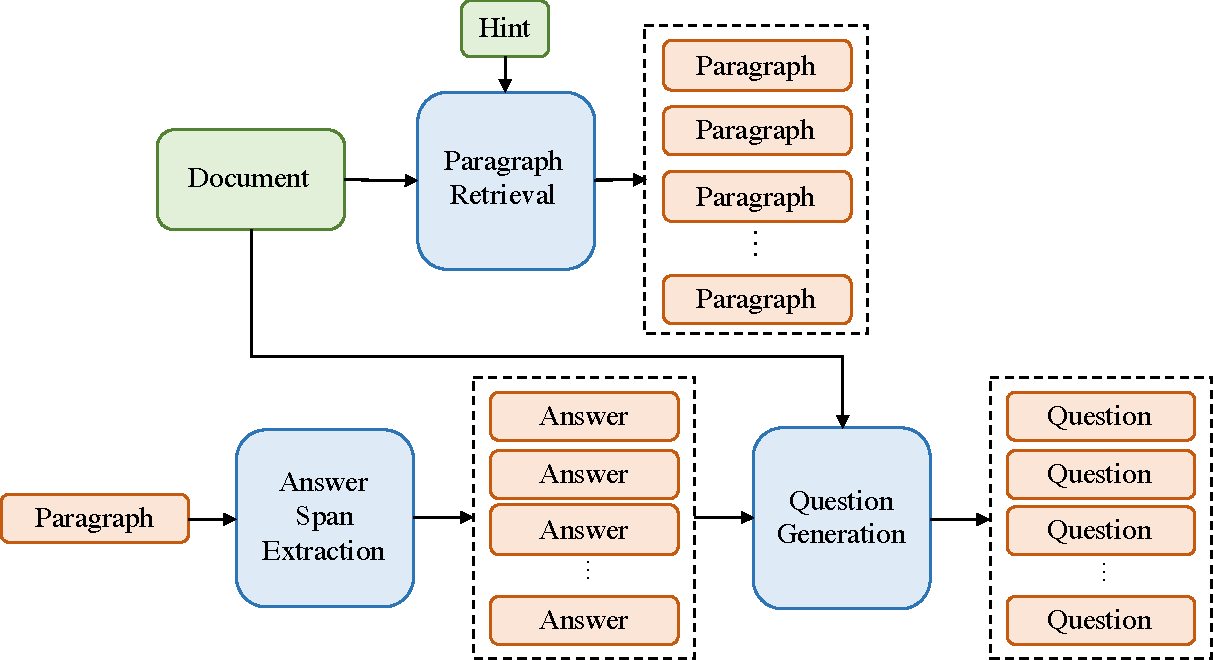
\includegraphics[width=0.45\textwidth]{pic/pipeline.pdf}
		\caption{\label{fig:pipeline} An overview of the pipeline process by which we generate QA pairs from the document. It consists of the feeding input data shown in blue blocks, the retrieval module, answer extraction module and question generation module which are blocked in orange, and the intermediate and final results in green blocks.}
	\end{center}
\end{figure}

\subsection{Filtering Method}
The process of filtering method is shown as Figure \ref{fig:filtering}. In filtering method, we choose all paragraphs in the document in the Paragraph Retrieval step, and generate the QA pairs in the same way as Section \ref{sec:pipeline}. The difference is that there exists a filtering process after QA pairs are generated, we omit QA pairs that are not relevant to the hint. In this case, QA pairs related to the hint is not limited to the certain paragraphs.

\begin{figure}[th]
	\begin{center}
	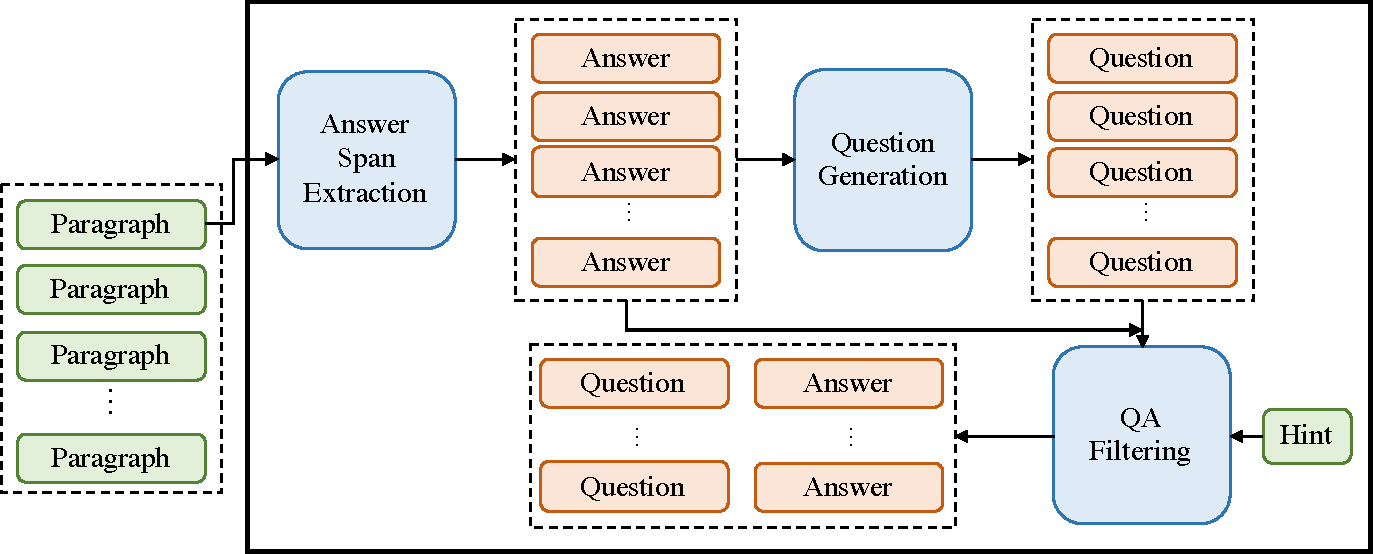
\includegraphics[width=0.45\textwidth]{pic/filtering.pdf}
		\caption{\label{fig:filtering} An overview of the filtering process by which we generate QA pairs from the document. Note that only one paragraph is blocked for clarity.}
	\end{center}
\end{figure}

\subsection{Joint Model: AspectQAG}
% Inspired by the pre-trained language model UNILM~\cite{dong2019unified} which shares the Transformer~\cite{vaswani2017attention} with respect to bidirectional LM, unidirectional LM, and sequence-to-sequence LM, we fine tune our AspectQAG containing all of these LMs which is shown as Figure \ref{fig:joint}.

Sharing parameters in close tasks is a effective method in Deep Learning. In this task, the embedding for paragraph and hint can be reused in answer extraction and question generation, and we proposed a joint model to reuse this embedding. The proposed model is called ``AspectQAG'', we show the architecture of the model in Figure~\ref{fig:joint}.

\begin{figure}[th]
	\begin{center}
	\includegraphics[width=0.5\textwidth]{pic/joint-2.eps}
		\caption{\label{fig:joint} An overview of AspectQAG. We pack the segments of paragraph and hint together for simplicity because they have the same LM structure. Actually, there is a [SEP] token between the two segments. For Classifier Loss, we only consider the paragraph segment in $PH$. Same as UNILM, we use the self-attention mask to control the access to context for each token.}
	\end{center}
\end{figure}

% As a joint model, AspectQAG is trained with two losses: the classifier loss for answer extraction and the generation loss for question generation. At test time, AspectQAG can extract answers with the input of paragraph and hint first, and then generate questions with the input of paragraph, hint and extracted answers.

During training time, the input of AspectQAG is a sequence of tokens which consists of three parts: the segments of the paragraph and hint ($S_{PH}$), the segment of the answer ($S_{A}$) and the segment of the question ($S_{Q}$). 
Training loss of the joint model has two major components, they are the classifier loss for answer extraction and the generation loss for question generation.
% This joint model realizes the answer extraction and question generation at the same time. The details are as follows.

\paragraph{Paragraph Retrieval.} We add irrelevant (paragraph, hint) pairs into the training data, the ground truth answers and questions of these irrelevant pairs are empty. The proportion of relevant and irrelevant (paragraph, hint) pairs is 5:1.

\paragraph{Answer Extraction.} The contradiction between answer extraction and question generation is that the former does not take answers as input, but the latter requires it. Our solution is to mask the attention of the $S_{A}$ for $S_{PH}$ and take the transformer output of $S_{PH}$ to train the classifier. The output of the paragraph segment will go through a linear layer to give predict the label of each token in the paragraph among 'O', 'B', and 'I' (Note that the hint is document independent, so we only mark the labels in paragraph area). We obtain classifier loss by calculate the cross entropy of the prediction and ground truth labeled sequence.

% As shown in Figure \ref{fig:joint}(b), this module is related to the area of $S_{PH}$ 
% %which is shown in Figure \ref{fig:joint}(b).
% where only the paragraph and hint are available .
% We choose the unidirectional LM to support the sequence labeling for answer span extraction with label of `O', `B' and `I'.
% Note that the hint is document independent, so we only mark the labels in paragraph area.

\paragraph{Question Generation.} During question generation, the answer segment $S_A$ is considered as the source sequence together with $S_{PH}$, and the question segment $S_Q$ is regarded as the target sequence. We randomly mask 80\% tokens in the question segment $S_Q$, and learn to predict the masked token during training time. Since the output sequence is unknown at test time, we follow the decoder of seq2seq structure and use a left-to-right attention mask in segment $S_Q$. We take the loss of masked token prediction as the generation loss. 

% In this module, the answer segment $S_A$ is considered as the source sequence together with $S_{PH}$, and the question segment $S_Q$ is regarded as the target sequence.
% Because $S_A$ is invisible in answer extraction module, there is a bidirectional LM for $S_A$ but a left-to-right unidirectional LM between $S_{PH}$ and $S_A$.
% In order to follow the principle of sequence-to-sequence structure, there is a left-to-right unidirectional LM which allows the context of to-be-predicted token in $S_Q$ contains all the tokens in $S_{HP}$ and $S_A$, and the tokens on its left.

For overall training, we calculate the final loss as the synthesis of the answer extraction and question generation. We add two losses at a certain ratio as the final loss for training.
\begin{equation}
    Loss = Loss_{classifier} + \lambda \cdot Loss_{generation}
\end{equation}

% \SY{loss function}

At test time, we take all paragraphs in the input document as the input and generate QA pairs in two steps. The first step is to extract answer spans with the classifier taken paragraph and hint as input. If the result is an empty set, we consider the input paragraph and hint as irrelevant, otherwise, we continue to the second step and generate questions with the generation component taken paragraph, hint and the extracted answers as input.